\section{Odometry}
%=========================================================================================================================
%-------------- MOTOR CONTROL
%=========================================================================================================================
\subsection{Motor Control}
As each wheel spins the sensor will gather data about the angular position change of the wheel. Once the encoder input has been captured it must be converted to linear velocity and used by a robotic kinematic model to create an estimate of the distance traveled and possible error.
Two wheel encoders are used to deduce the speed and travel direction by measuring the number of pulses registered from each wheel. Each wheel encoder has two sensors and is capable of
registering a distance resolution of 1/36th of the robot’s wheel circumference.
The Position Controllers on Eddie use a quadrature encoder system to reliably track the position and speed of each wheel at all times. With the included plastic encoder disks, each Position Controller has a resolution of 36 positions per rotation; this equates to approximately 0.5 inches of linear travel per position using the included 6 inch tires. 
The Position Controllers calculate and report position and average speed data on command.
Knowing that the sensor has 1/36th resolution of wheel circumference, the sensor produces 36 pulses for every complete revolution of the wheel. Based on this, the distance traveled
in the duration of one pulse is given below:
\begin{equation}\label{eq:1}
    d=\frac{2\pi r}{36} \\
\end{equation}
\lstinputlisting[caption=eddie\_controller.cpp, label={lst:listing-cpp}, language=C++]{code/eddie_controller.cpp}
%=========================================================================================================================
%-------------- WHEEL ODOMETRY MODEL
%=========================================================================================================================
\subsection{Wheel Odometry Model}
With the rotation data, alongside information on the encoder, such as the radius or circumference, we can estimate the distance traveled by the wheel. Since each slit represents some angle of rotation, knowing the number of slits passed informs us about the amount of rotation between time steps. For an optical encoder, where all the slits are equally spaced, we could get the total angle of rotation between time steps by multiplying the number of slits passed by the amount of rotation represented by a single slit. After we determine the angle of rotation, we can multiply it by the circumference of the encoder to get the distance traveled by the wheel.

The goal of an odometry model is to estimate the position and orientation of the robot. To achieve this, we’ll leverage data from the rotary encoders, the dimensions of our robot, and geometry. The encoder will inform us of the distance traveled by each wheel at each time step. In terms of using the dimensions of our robot, the only dimension we need is the distance of the point from the left and right wheels. Since we defined our reference point to be located equidistant between the two wheels, we only need to keep track of one number.\\

Now let’s define some variables to keep track of these ideas:
\begin{figure}[H]
	\centering
	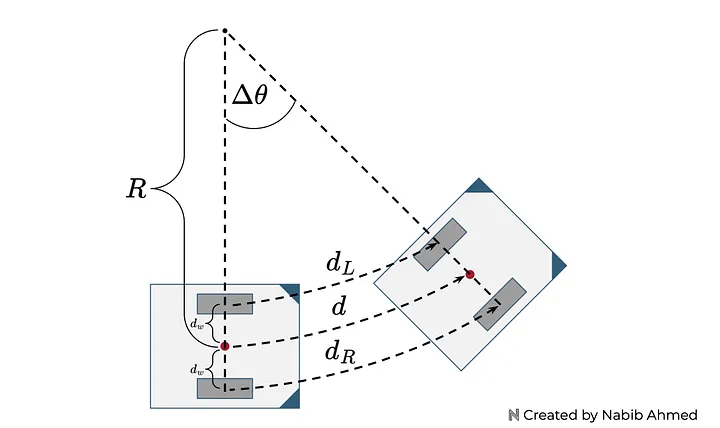
\includegraphics[width=0.8\linewidth]{figures/odom.png}
	\caption{}
	\label{fig:odom}
\end{figure}

\quad \quad $d_L$ = distance traveled by the left wheel.

\quad \quad $d_R$ = distance traveled by the right wheel.

\quad \quad $d_w$ = distance between the reference point and the wheels.

\quad \quad $d$ = distance traveled by the reference point.

\quad \quad $\Delta \theta$ = A change in the angle of rotation.

\quad \quad $R$ = radius of the curve containing the reference point.\\

$d_L$ and $d_R$ correspond to the distance traveled by the wheel at a certain time step. This information will come from our rotary encoder. $d_w$ can be derived by measuring the distance between the two wheels and dividing it in half since the point is equidistant from the two wheels. The last three variables are not directly measurable — instead, we need to use geometry to relate these variables to the measurable quantities.\\

We can start by using the arc length formula. The path for the left wheel, right wheel, and reference points are arcs. They all share the same angle and the radius for each can be expressed in terms of the radius of the curve containing the reference point and the distance between the reference point and the wheels.
\begin{equation}\label{eq:2}
    d =  R\Delta \theta\\
\end{equation}
\begin{equation}\label{eq:3}
    d_L = (R-d_w)\Delta \theta\\
\end{equation}
\begin{equation}\label{eq:4}
    d_R = (R+d_w)\Delta \theta
\end{equation}
Now we solve for the change in the angle of rotation in terms of measurable quantities, getting the following relationship:
\begin{equation}\label{eq:5}
    \Delta \theta = \frac{d_R - d_L}{2d_w}
\end{equation}
Now we solve for the radius of the curve containing the reference point by rearranging equations and plugging in what we know. Then, we solve for the distance travelled by the reference point.
\begin{equation}\label{eq:6}
    R = d_L \frac{2d_w}{d_R - d_L}+d_w
\end{equation}
\begin{equation}\label{eq:7}
    d = \frac{d_R + d_L}{2}
\end{equation}

We solved for all variables in terms of measurable quantities. Since we’re interested in the robot’s position and orientation, the key variables of interest would be the distance traveled by the reference point and the change in the angle of rotation. The distance traveled by the reference point informs us of the position and the change in the angle of rotation informs us of the orientation. The radius of the curve containing the reference point, while useful for derivation, is not really needed anymore.\\

Now, we know the distance traveled, but not the direction. We know how much the orientation angle changed, but not the new orientation angle. So we start modifying our odometry model.\\

To simplify our model, we will represent the distance traveled by the reference point as a line instead of a curve.
We can make this simplification because typically, in wheel odometry with encoders, the data sampling is very high. What this means is that our encoders are able to collect data very frequently so the time window between measurements is very small. Since the time window is very small, the amount of motion captured by each time step will also be small. For our model, that means the curvature of the arc will be very small and resemble a straight line. Thus, it’s a safe assumption and simplification to represent our distance now as a straight line. We then calculate the angle of the distance in terms of a previously solved variable, and the new orientation of the robot as shown in Figure \ref{fig:alphabeta}:
\begin{figure}[H]
	\centering
	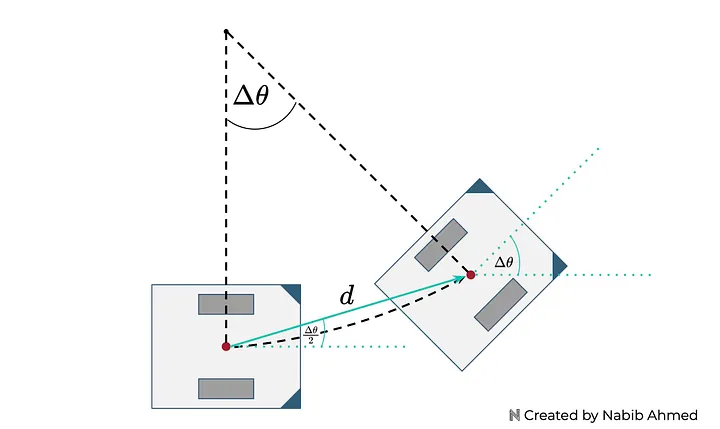
\includegraphics[width=0.8\linewidth]{figures/alpha beta.png}
	\caption{}
	\label{fig:alphabeta}
\end{figure}

In Figure \ref{fig:thetat}, the odometry model at time $t$ will add the absolute orientation angle from the previous time step. Notice that adding the orientation from the previous time step won’t change the distance traveled by the reference point or the change in angle of rotation as the formulas we derived from earlier don’t rely on the orientation angle (only the traveled wheel distances). Instead what does change is the orientation of the robot, from being relative between time steps to now being absolute on the coordinate plane. Thus, the absolute orientation angle at any time step can be defined by:
\begin{equation}\label{eq:8}
    \theta_t = \theta_{t-1} + \Delta \theta_t
\end{equation}\\
\begin{figure}[H]
	\centering
	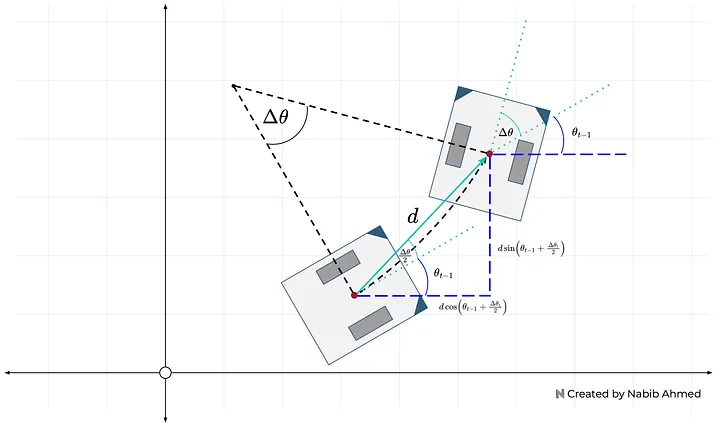
\includegraphics[width=0.8\linewidth]{figures/theta t.png}
	\caption{}
	\label{fig:thetat}
\end{figure} 

Using the distance traveled by the reference point and the angle of orientation from the previous time step plus the angle that results from motion, the amount of distance traveled along the x and y directions can be calculated.
\begin{equation}\label{eq:9}
    x_t = x_{t-1} + d cos(\theta_{t-1} + \frac{\Delta \theta_t}{2})
\end{equation}\\
\begin{equation}\label{eq:10}
    y_t = y_{t-1} + d sin(\theta_{t-1} + \frac{\Delta \theta_t}{2})
\end{equation}\\
\begin{figure}[H]
	\centering
	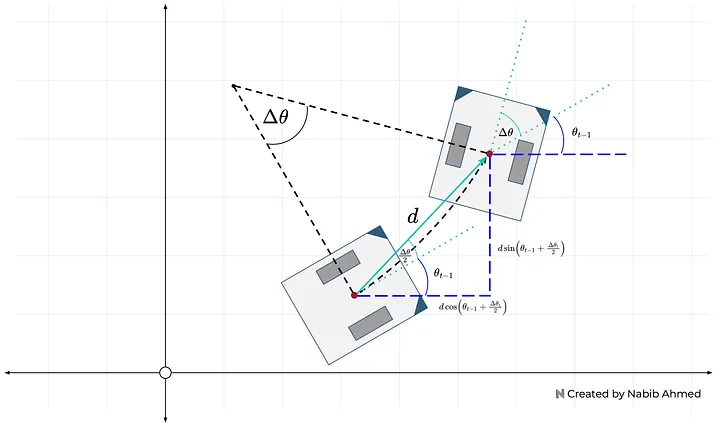
\includegraphics[width=0.8\linewidth]{figures/xtyt.png}
	\caption{}
	\label{fig:xtyt}
\end{figure} 
\lstinputlisting[caption=eddie\_odom.cpp, label={lst:listing-cpp}, language=C++]{code/eddie_odom.cpp}

